\chapter{Компьютерное моделирование}
\label{ch:chap1}

\section{Моделирование в Matlab/Simulink}

В программной середе Matlab/Simulink была сделана модель по системе
уравнений \eqref{eq:system}. Ниже представлены фото модели 
и графики моделирования при разных подаваемых напряжениях 
на электродвигатели. Модели бесколлекторных электродвигателей
были созданы на основе моделей представленных в \cite{article}.

\subsection{Модель}


\begin{figure}[ht]
    \centering
    \includegraphics[width=1 \textwidth]{model-11.png}
    \caption{Модель в общем виде}
    \label{fig:model-1}
\end{figure}

\begin{figure}[ht]
    \centering
    \includegraphics[width=1 \textwidth]{model-10.png}
    \caption{Модель в общем виде}
    \label{fig:model-2}
\end{figure}

\newpage

\subsection{Графики моделирования}

\begin{figure}[ht]
    \centering
    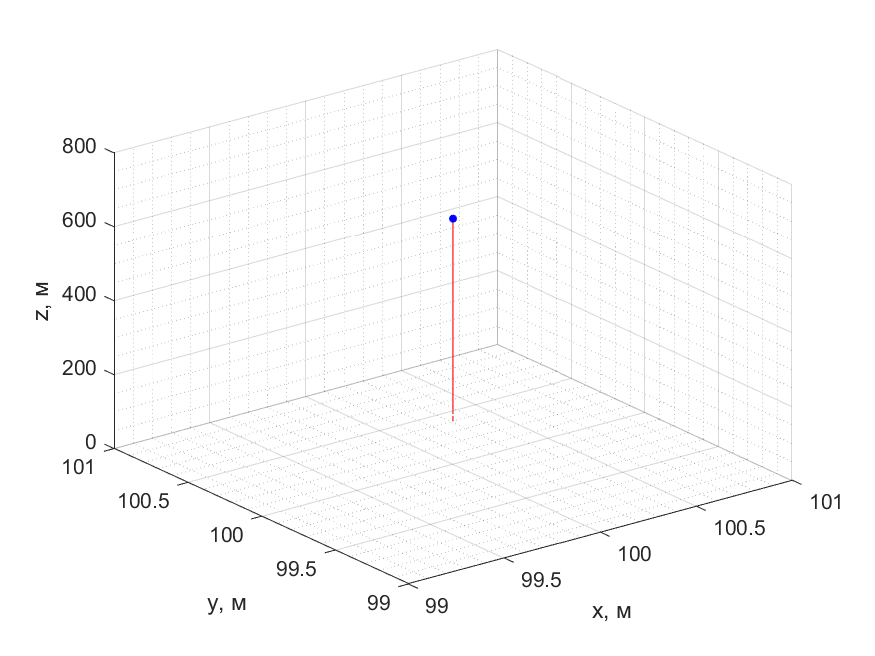
\includegraphics[width=0.75 \textwidth]{modeling_v_0_1_1.png}
    \caption{График моделирования квадрокоптера при входных напряжениях: \(U_1=5.5\)В, \(U_2=5.5\)В, \(U_3=5.5\)В, \(U_4=5.5\)В. Внешнее сопротивление отсутствует.}
    \label{fig:modeling-1}
\end{figure}

\begin{figure}[ht]
    \centering
    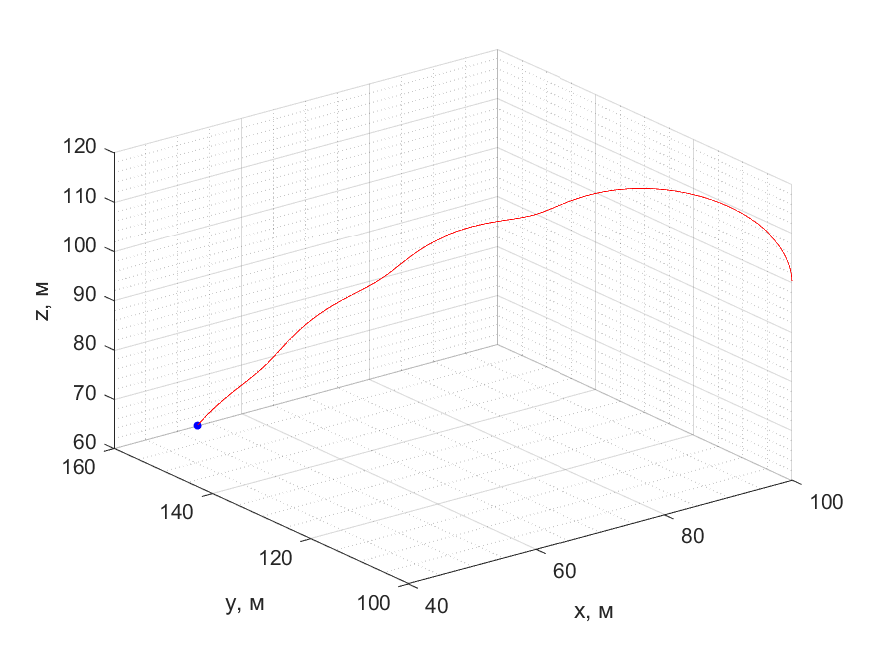
\includegraphics[width=0.75 \textwidth]{modeling_v_0_1_2.png}
    \caption{График моделирования квадрокоптера при входных напряжениях: \(U_1=5.5\)В, \(U_2=5.5\)В, \(U_3=0\)В, \(U_4=0\)В. Внешнее сопротивление отсутствует.}
    \label{fig:modeling-2}
\end{figure}

\begin{figure}[ht]
    \centering
    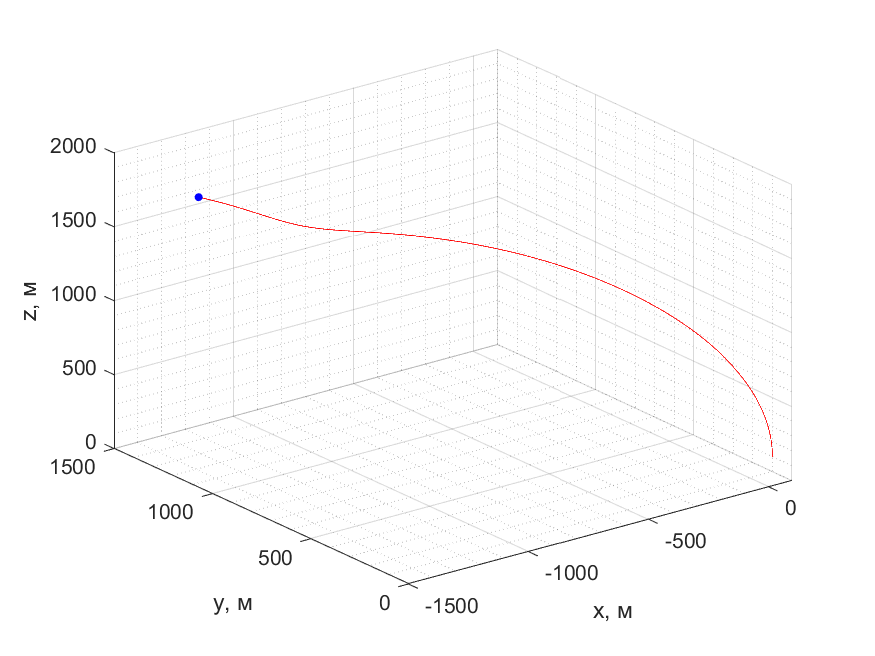
\includegraphics[width=0.8 \textwidth]{modeling_v_0_1_3.png}
    \caption{График моделирования квадрокоптера при входных напряжениях: \(U_1=5.5\)В, \(U_2=5.5\)В, \(U_3=5.4\)В, \(U_4=5.4\)В. Внешнее сопротивление отсутствует.}
    \label{fig:modeling-3}
\end{figure}

\begin{figure}[ht]
    \centering
    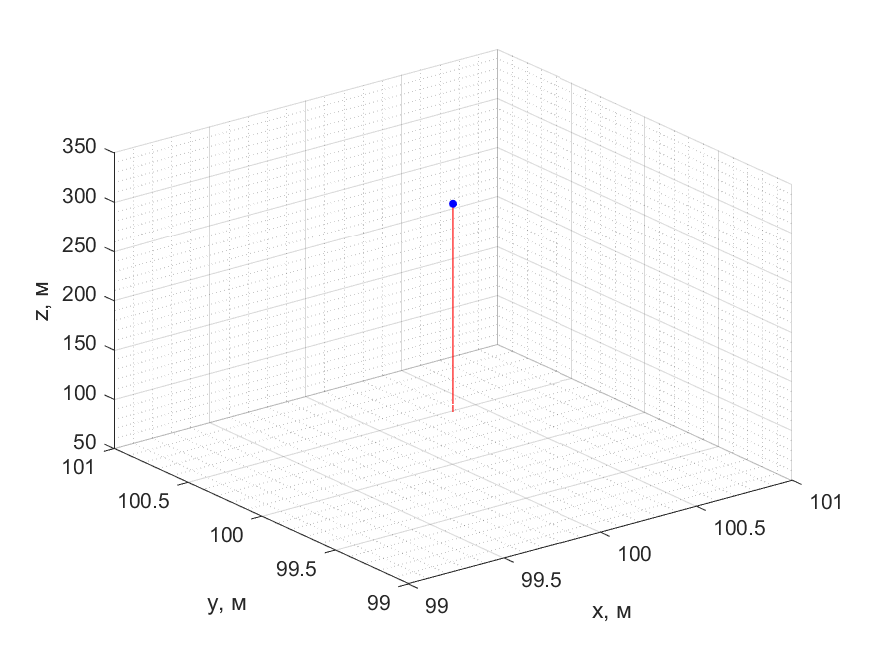
\includegraphics[width=0.8 \textwidth]{modeling_v_0_1_4.png}
    \caption{График моделирования квадрокоптера при входных напряжениях: \(U_1=5.5\)В, \(U_2=5.5\)В, \(U_3=5.5\)В, \(U_4=5.5\)В. Коэффициенты внешних сопротивлений \(C_a=C_b=0.1\), \(C_{drag}=1.1\).}
    \label{fig:modeling-4}
\end{figure}

\begin{figure}[ht]
    \centering
    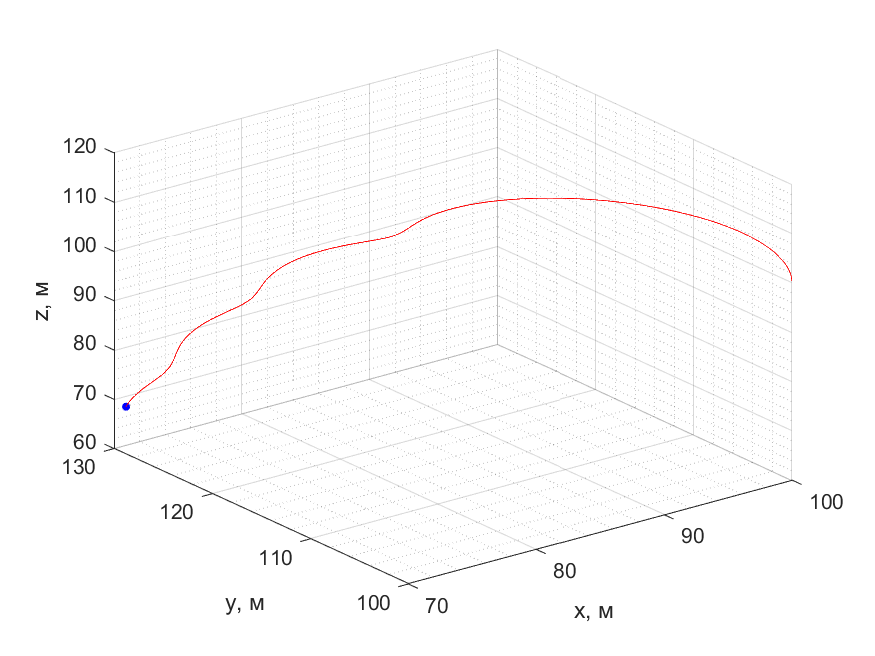
\includegraphics[width=0.8 \textwidth]{modeling_v_0_1_5.png}
    \caption{График моделирования квадрокоптера при входных напряжениях: \(U_1=5.5\)В, \(U_2=5.5\)В, \(U_3=0\)В, \(U_4=0\)В. Коэффициенты внешних сопротивлений \(C_a=C_b=0.1\), \(C_{drag}=1.1\).}
    \label{fig:modeling-5}
\end{figure}


\begin{figure}[ht]
    \centering
    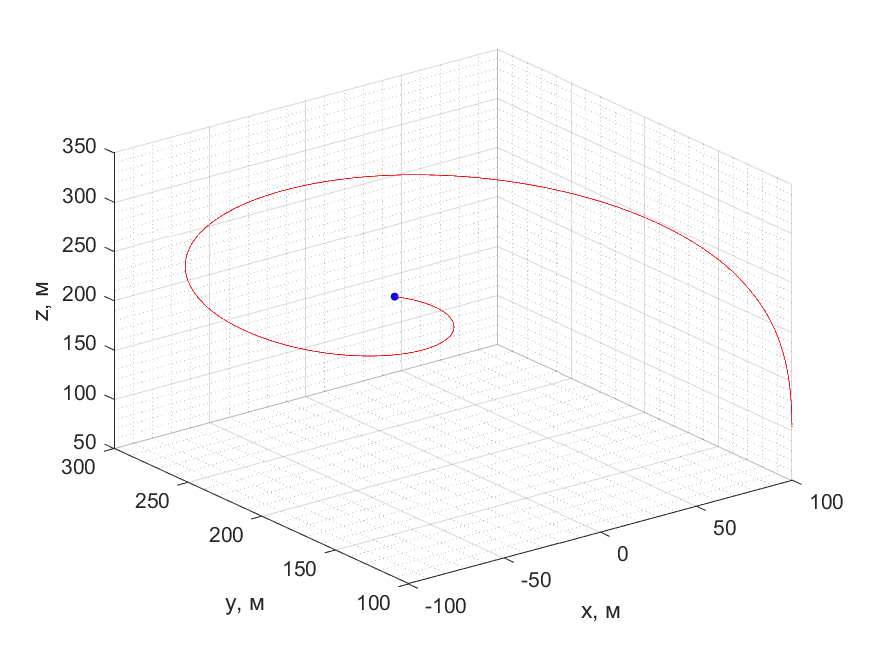
\includegraphics[width=0.8 \textwidth]{modeling_v_0_1_6.png}
    \caption{График моделирования квадрокоптера при входных напряжениях: \(U_1=5.5\)В, \(U_2=5.5\)В, \(U_3=5.4\)В, \(U_4=5.4\)В. Коэффициенты внешних сопротивлений \(C_a=C_b=0.1\), \(C_{drag}=1.1\).}
    \label{fig:modeling-6}
\end{figure}


\section{Моделирование в САПР Solidworks}

Также была создана модель квадрокоптера в САПР Solidworks.
Многие компоненты модели были найдены в интернете в свободном
доступе. В дальнейшем планируется добавить САПР модель
квадрокоптера в Simulink для более точного и наглядного 
моделирования.

\subsection{Фотографии квадрокоптера}

\begin{figure}[ht]
    \centering
    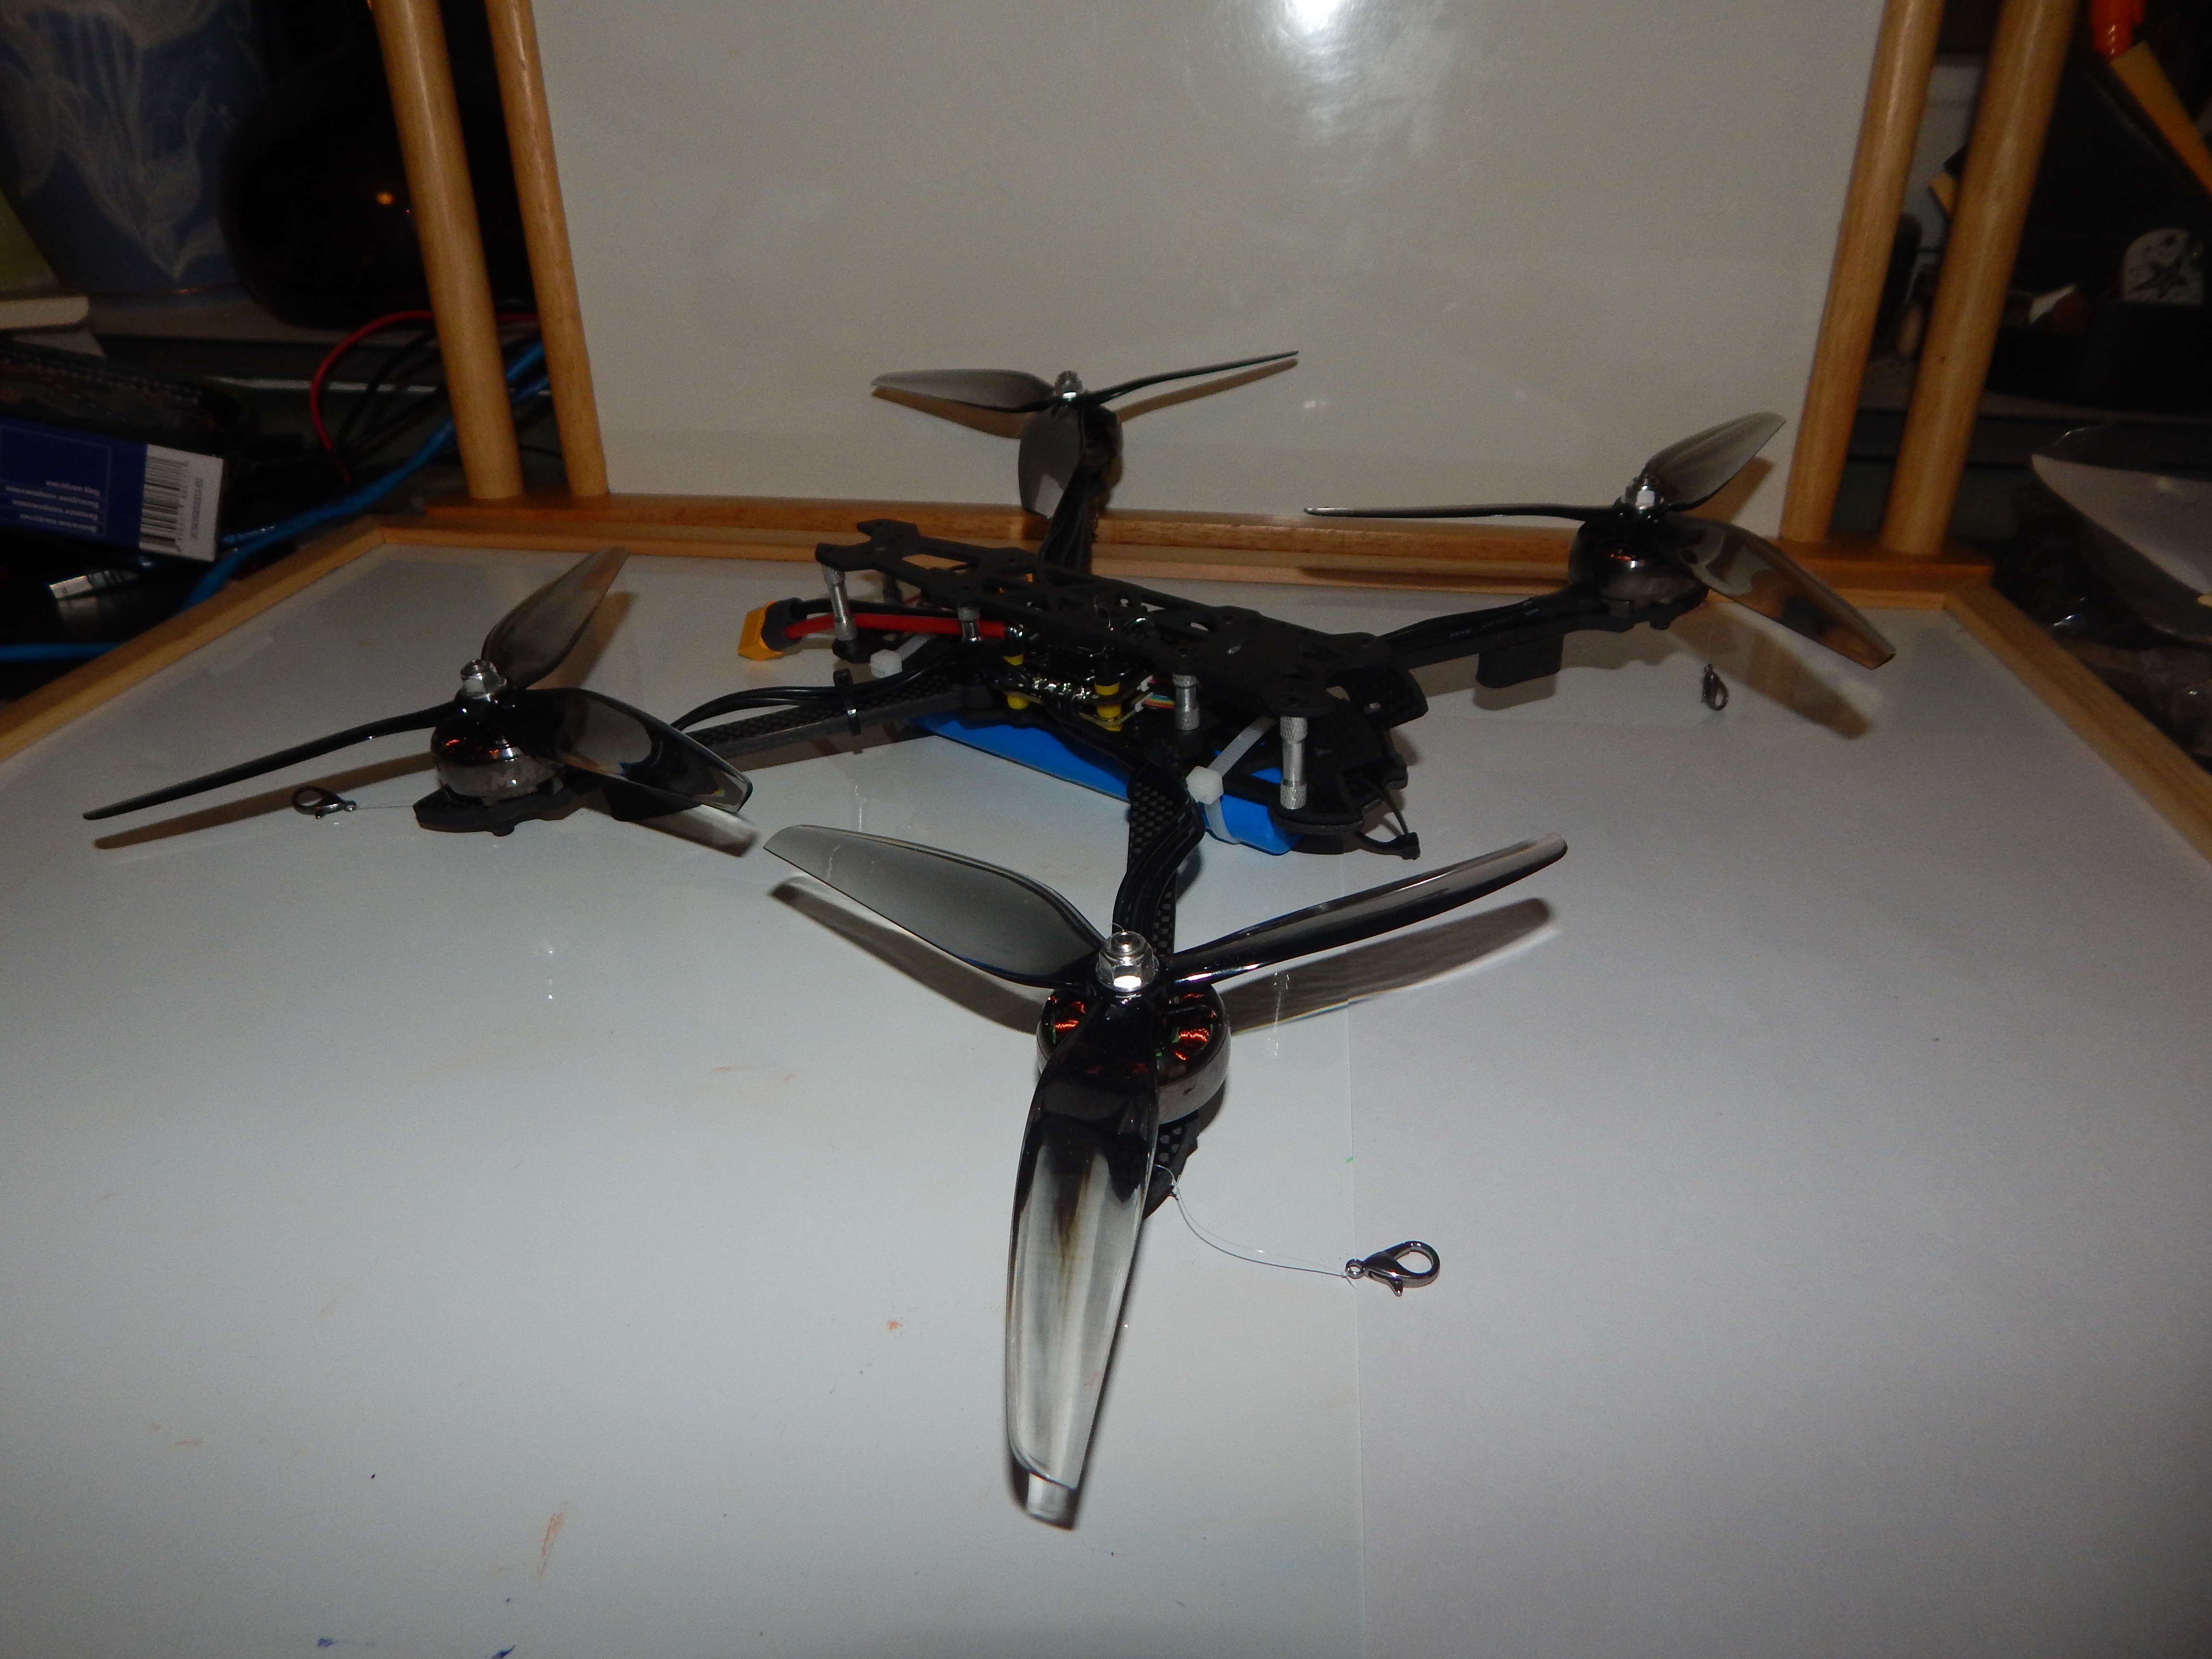
\includegraphics[width=0.8 \textwidth]{DSCN0425.JPG}
    \caption{Фотография квадрокоптера}
    \label{}
\end{figure}

\newpage

\subsection{Модель САПР}

\begin{figure}[ht]
    \centering
    \includegraphics[width=0.8 \textwidth]{cad-model-1.png}
    \caption{Модель квадрокоптера в Solidworks}
    \label{}
\end{figure}


\endinput